% document type
\documentclass[12pt]{article}

\usepackage[a4paper, includefoot,
            left=3cm, right=1cm,
            top=1.5cm, bottom=1.5cm,
            headsep=1cm, footskip=1cm]{geometry}
%Russian-specific packages
%--------------------------------------
\usepackage[T2A]{fontenc}
\usepackage[utf8]{inputenc}
\usepackage[russian]{babel}
%--------------------------------------
 
%Hyphenation rules
%--------------------------------------
\usepackage{hyphenat}
\usepackage{tempora}

% в преамбуле
\usepackage{subcaption}

\usepackage{physics}
\usepackage{fixint}
\usepackage{tikz}
\usepackage{hyperref}
\usepackage{graphicx} % для вставки картинок
\usepackage{amssymb,amsfonts,amsmath,amsthm} % математические дополнения от АМС
\usepackage{indentfirst}
\usepackage{nicefrac,xfrac}
\usepackage{subcaption}

\usepackage{cmap}

\linespread{1.3} % полуторный интервал
\frenchspacing

\newcommand*{\figref}[2][]{\hyperref[#2]{Рис.~\ref*{#2}#1}}
\newcommand*{\tabref}[2][]{\hyperref[#2]{Табл.~\ref*{#2}#1}}
% \newcommand*{\tblref}[1]{\hyperref[#1]{Table~\ref*{#1}}}
\newcommand*{\secref}[1]{\hyperref[#1]{Section~\ref*{#1}}}
% \newcommand*{\secsref}[1]{\hyperref[#1]{Sections~\ref*{#1}}}
% \newcommand*{\introref}[1]{\hyperref[#1]{Introduction}}

\begin{document}
	\begin{titlepage}
    \begin{center}
    % \vspace{-3em}
    {\small\textsc{Нижегородский государственный университет имени Н.\,И. Лобачевского}}
    \vskip 2pt \hrule \vskip 3pt
    {\small\textsc{Высшая школа общей и прикладной физики}}

    \vfill


    {{\large Отчет по лабораторной работе}\vskip 12 pt {\Large \bfseries ВОЛЬТ-АМПЕРНЫЕ ХАРАКТЕРИСТИКИ ДИОДОВ ШОТТКИ}}

        
    \vspace{2cm}
    {\large Работу выполнили студенты \\[0.5em]{\Large \bfseries Поляков Андрей, Козлов Александр}}

    \end{center}

    \vfill

    \begin{center}
    {Нижний Новгород, \today}
    \end{center}
\end{titlepage}
	\setcounter{page}{2}

	\tableofcontents
	\newpage

	\section{Вольт-амперная характеристика диода Шоттки}
	Измерили вольт-амперную характеристику (ВАХ) диодов Шоттки при различных температурах. Первым делом обсудим температуру. Температура определялась по напряжению на термопаре "{}медь-константан"{} и постоянно менялась. Чтобы перевести напряжение термопары в температуру, надо было воспользоваться градуировочной таблицей из методички, что мы и сделали с помощью кусочно-линейной аппроксимации данных таблицы.

	Изначально ток измерялся в Амперах, но для соотнесения с теорией необходимо было перейти к плотности тока. Для этого использовалось знание о том, что поперечная площадь образца $S=0.5\,\textnormal{мм}^2$.

	На \figref{fig:j_vs_v} представлены снятые ВАХ диода Шоттки. Видно, что все измерения снимались при условии $V > kT/e$. Из теории известно, что плотность тока зависит от напряжения следующим образом
	\begin{equation}
		j = j_0 \qty(\exp{\dfrac{eV}{kT}} - 1),
	\end{equation}
	где 
	\begin{equation}
		j_0 = A^* T^2 \exp{-\dfrac{e\varphi_b}{kT}}.
	\end{equation}
	Здесь $A^*=4\pi m^* e k^2/h^3$ --- эффективная постоянная Ричардсона, $\varphi_b$ --- высота потенциального барьера Шоттки.

	\begin{figure}[htbp]
		\centering
		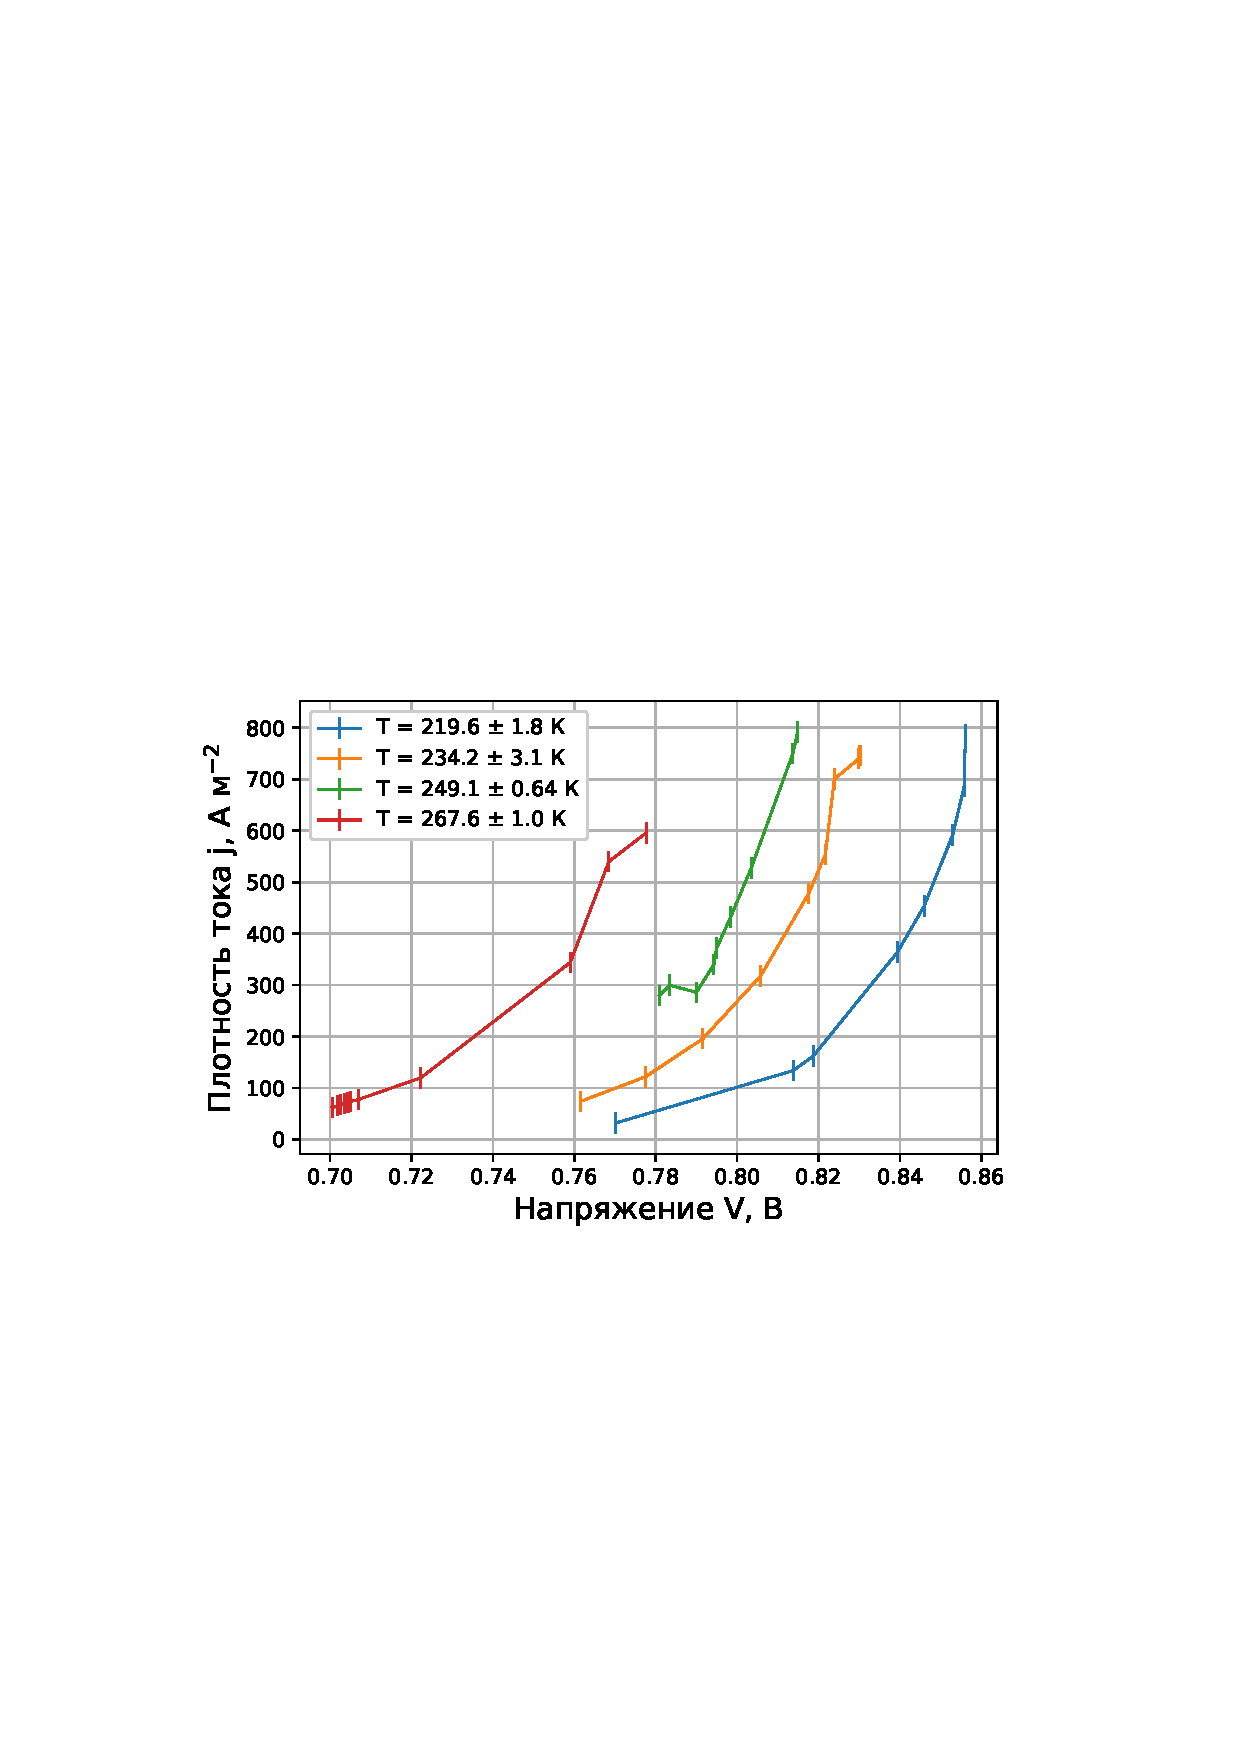
\includegraphics[width=\textwidth]{../figures/j_vs_v.png}
		\caption{Семейство ВАХ диода Шоттки при различных температурах. Измерительная погрешность тока взята за 0.1 мА.}
		\label{fig:j_vs_v}
	\end{figure}

	\section{Определение эффективной постоянной Ричардсона, эффективной высоты потенциального барьера Шоттки и эффективной массы электрона}

	Для того, чтобы определить эффективную постоянную Ричардсона $A^*$ и эффективную высоту потенциального барьера Шоттки $\varphi_0 = \varphi_{b0} - \Delta \varphi_{b0}$, была построена на основе экспериментальных данных зависимость $\mathrm{ln}\{ j\,/\, [1 - \mathrm{exp}(-eV\,/\,kT)] \}$ от $V$ (см. \figref{fig:bigeq_vs_v}).

	\begin{figure}[htbp]
		\centering
		\includegraphics[width=\textwidth]{../figures/bigeq_vs_v.png}
		\caption{Зависимость $\mathrm{ln}\{ j\,/\, [1 - \mathrm{exp}(-eV\,/\,kT)] \}$ от $V$ при различных температурах. Погрешности рассчитаны стандартным образом.}
		\label{fig:bigeq_vs_v}
	\end{figure}

	Каждая из таких зависимостей аппроксимировалась прямой и находился свободный коэффициент линейной регрессии, который равен $\mathrm{ln}j_0$. Это позволило определить зависимость $j_0$ от температуры. Далее строилась зависимость $\mathrm{ln}\{j_0\, /\, T^2\}$ от $1\,/\,T$  и опять же делалась линейная регрессия (см. \figref{fig:ln_vs_1T}). Старший коэффициент в такой линейной регрессии равен $-e\varphi_0/kT$, а свободный --- $\mathrm{ln}A^*$, откуда требуемые значения и находились.

	\begin{figure}[htbp]
		\centering
		\includegraphics[width=\textwidth]{../figures/ln_vs_1T.png}
		\caption{Зависимость $\mathrm{ln}\{j_0\, /\, T^2\}$ от $1\,/\,T$.}
		\label{fig:ln_vs_1T}
	\end{figure}

	Итоговые значения с учётом погрешностей метода наименьших квадратов, который использовался для линейной регрессии, получились следующими:
	\begin{equation}
		A^* = (7.3 \pm 10.3)\times10^3\:\textnormal{A м}^{-2}\textnormal{ к}^{-2};\quad \varphi_0 = 0.80\pm0.03\: \textnormal{В}.
	\end{equation}
	Отсюда находим, что $m^*/m = 0.006 \pm 0.009$.

	\section{Определение фактора неидеальности диода Шоттки}
	Для определения фактора неидеальности диода Шоттки $n$ была использована следующая формула
	\begin{equation}
		 n = \frac{ej}{kT\; \mathrm{d}{j}\,/\,\mathrm{d}{V}}.
	\end{equation}
	Данный фактор был рассчитан для каждой ВАХ. Все значения были собраны в один массив, затем было вычислено среднее значение по массиву, а так же стандартное отклонение, что дало ответ $n = 1.24 \pm 0.51$.

\end{document}